\documentclass[11pt, oneside]{article} 
\usepackage{geometry}
\geometry{letterpaper} 
\usepackage{graphicx}
	
\usepackage{amssymb}
\usepackage{amsmath}
\usepackage{parskip}
\usepackage{color}
\usepackage{hyperref}

\graphicspath{{/Users/telliott/Github/precalculus/fig/}}

\title{Quadrilaterals}
\date{}

\begin{document}
\maketitle
\Large

Quadrilaterals are four-sided figures.  There are a number of types, some of which are:

$\bullet$ square:  four sides equal, four right angles 

$\bullet$ rectangle:  opposite sides equal, four right angles

$\bullet$ rhombus:  all sides equal, opposite sides parallel

$\bullet$ parallelogram: opposite sides equal and parallel

$\bullet$ trapezoid: two sides parallel

$\bullet$ kite: adjacent sides equal

\subsection*{parallelogram}

Let's look at parallelograms, which can be viewed as two congruent triangles that have been stitched together.

\begin{center} 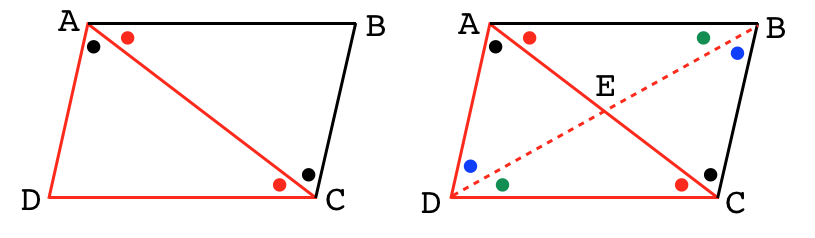
\includegraphics [scale=0.4] {pgram1.png} \end{center}

The definition of a parallelogram is that it is a four-sided figure with opposing sides of equal length and parallel.  Thus, the interior angles theorem gives us the angle equalities shown.  

On the left, we have three angles the same and a shared side, hence $\triangle ABC \cong \triangle ACD$.

Therefore, $AB = DC$ and $AD = BC$.

If we draw the other diagonal and change nothing else, the two triangles are congruent by ASA.  

An important property of parallelograms follows:  the diagonals cross at their midpoints.

\subsection*{rhombus}

If we further constrain all the sides to be equal, then the half triangles like $\triangle ADC$ become isosceles.  

The isosceles triangle theorem says that in a triangle with two sides equal the base angles are equal.  The converse is also true.

By the isosceles triangle theorem, all the angles marked with red dots are equal, and all the blue ones as well.  Because each quarter triangle has a red and a blue, the central angles are all equal.  Therefore, they are all right angles.

\begin{center} 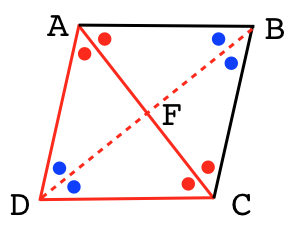
\includegraphics [scale=0.4] {pgram2.png} \end{center}

Now, finally, let us assemble one whole and two have parallelograms starting with the same figure.

\begin{center} 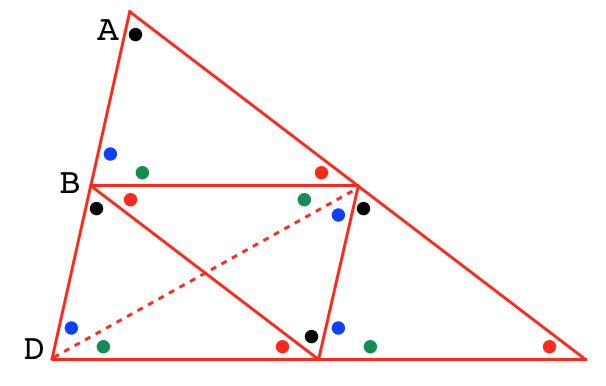
\includegraphics [scale=0.4] {pgram4.png} \end{center}

By the properties of the parallelogram, if the adjacent sides $AB$ and $BD$ are equal, all the angles work out and we get four congruent triangles, so the adjacent sides of the large triangle all have equal segments as well.

\end{document}